\section*{Introducción}
\addcontentsline{toc}{section}{Introducción}
\subsection*{Necesidades de los sistemas para Big Data}
\addcontentsline{toc}{subsection}{Necesidades de los sistemas para Big Data}
Un sistema para Big Data necesita infraestructura que procese:
\begin{itemize}
	\item \textbf{Grandes cantidades de información.} Se estima que el volumen de datos que se genera globalmente al año crece un 41\%. 
	\item \textbf{Gran variedad de fuentes y formatos.} Se estima que el 80\% de los datos globales son desestructurados, es decir, no tienen la estructura típica de un csv (emails, texto plano, redes sociales, código, chats, fotos, vídeos, etc)
	\item \textbf{Con alta cadencia de entradas de datos}
	\item \textbf{Con flexibilidad y uso eficiente de recursos}. Una de las principales tendencias es la virtualización y el dimensionamiento de recursos en tiempo real (On-Premise o Cloud).
\end{itemize}
Además, es buena práctica que el sistema sea capaz de integrar todo el ciclo de vida del dato: captura, preparación, enriquecimiento, análisis, modelización y mantenimiento.
\subsection*{Frameworks más utilizados}
\addcontentsline{toc}{subsection}{Frameworks más utilizados}
Los frameworks más populares son \textbf{Hadoop Mapreduce} y \textbf{Spark}. El sistema de ficheros que sustenta estas aplicaciones es \textbf{HDFS} y la base de datos distribuida más común es \textbf{Hbase} (Hadoop database).
\subsection*{HPC, Cloud Computing, Big Data y Deep Learning}
\addcontentsline{toc}{subsection}{HPC, Cloud Computing, Big Data y Deep Learning}
Conviene diferenciar bien estos cuatro conceptos que a menudo se mencionan juntos pero que pertenecen a realidades distintas.\\\\
\textbf{HPC (High Performance Computing)} hace referencia a la computación de altas prestaciones tradicional, basada en un cluster físico de computadores. Mientras que \textbf{Cloud computing} hace referencia al cómputo (de altas prestaciones o no) sobre infraestructura de terceros, habitualmente bajo demanda y de manera deslocalizada.
\textbf{Big Data} es el fenómeno que consiste en tratar grandes volúmenes de datos tan complejos que son necesarias técnicas computacionales y de análisis especializadas. \textbf{Deep Learning} es una rama del \textbf{Machine Learning} centrada en emular el proceso de pensamiento humano y es especialmente eficaz con grandes volúmenes de datos, de aquí su relación con el Big Data.
\break
\section{Clúster Hadoop}
Un clúster Hadoop es un tipo especial de clúster computacional específicamente diseñado para almacenar y analizar grandes volúmenes de datos no estructurados en un entorno de computación distribuída.
\subsection{Conceptos clave}
\begin{itemize}
	\item \textbf{Clúster para Big Data vs Clúster HPC.} Los clúster HPC están acotados por su capacidad de cómputo, ya que son difícilmente escalables y tienen un mayor ritmo de obsolescencia. Por otro lado, los clúster para Big Data están acotados por las comunicaciones entre nodos y acceso a los datos almacenados, ya que la información debe viajar entre nodos y es complicado leer y escribir de manera eficiente en disco.
	\item \textbf{Big Data, Cloud Computing y Virtualización}. Disponer de un clúster Big Data de manera permanente es muy costoso por lo que es común disponer de uno bajo demanda por varias razones: pago por uso (OPEX\footnote{Término contable o financiero que hace referencia a las inversiones operativas. Por lo general, la inversión en software se considera dentro del OPEX, algo que alivia la cifra total de inversión dentro del área de operaciones en el corto plazo. Por contra, la compra directa de hardware entra dentro del CAPEX o inversiones de capital, y su amortización contable debe estimarse (a menudo linealmente).}), flexibilidad o escalado.
	\item \textbf{Iaas y Paas}. Iaas (Infrastructure as a service) hace referencia a los servicios de computación cloud donde se pone a disposición del cliente recursos de computación virtualizados en un centro de datos (AWS, Azure, GCE, etc). Paas (Platform as a service) hace referecnia a los servicios que ponen a disposición del cliente, además de infraestructura, middleware, herramientas de desarrollo, servicios BI, administración de bases de datos, etc.
\end{itemize}
\subsection{Paradigma de ejecución de una aplicación}
Los datos por lo general se encuentran particionados en un \textbf{HDFS} desde el que se ingesta la información hacia la aplicación. Después de la ingesta, se ejecutan tareas Map de manera distribuída a cada nodo. Una vez aplicada la transformación Map, se realizan las operaciones Reduce para lograr el resultado deseado. En la figura \ref{fig:mapreduceexample} se ofrece un ejemplo de una aplicación para contar palabras.\\\\
La operación \textbf{map} consiste en una tarea individual que transforma un conjunto de pares clave-valor en otro conjunto de pares intermedios no necesariamente del mismo tipo que los originales.\\\\
La operación \textbf{reduce} consiste en una tarea individual que transforma pares clave-valor con la misma clave en un conjunto igual o menor de pares.\\\\
Entre el resultado del map y la ingesta del reduce existen tres tareas intermedias que pueden ejecutarse simultáneamente a medida que una tarea map produce resultados: \textit{shuffle}, \textit{combiner} y \textit{sort}.\\\\
Una tarea \textbf{shuffle} consiste en trasladar los pares clave-valor a la fase reduce. En este proceso, se pueden mezclar pares clave-valor de distintas particiones en una misma ingesta reduce. \textbf{Con esto se trata de evitar que un par clave-valor esté en varias particiones al mismo tiempo, lo que llevaría a un error en el cálculo.}\\\\
Una tarea \textbf{combiner} consiste en un reduce local, agregando valores con la misma clave usando la operación definida dentro de una misma partición. Esta fase ahorra tiempo de ejecución tanto en la fase de transferencia (disminuye el número de pares a transferir hacia el reduce) y en la fase sort del reduce (menos pares que ordenar).\\\\
Por último, la tarea \textbf{sort} consiste en agrupar todos los pares con la misma clave en una misma ingesta reduce.
\subsection{Modos de despliegue de Hadoop}
Hadoop se puede desplegar de tres maneras distintas:
\begin{itemize}
	\item \textbf{Standalone.} Las aplicaciones se ejecutan de manera local (como un único nodo), sin demonios, con entradas y salidas en el sistema de ficheros local (sin HDFS). Los principales usos son:
	\begin{enumerate}
		\item Debugging de aplicaciones
		\item Pruebas con la configuración por defecto
	\end{enumerate}
	\item \textbf{Pseudo-Distributed.} En este caso, las aplicaciones se ejecutan simulando un cluster. Los demonios se ejecutan en JVMs separadas (procesos java distintos). En este caso sí se usa HDFS. Los principales usos son:
	\begin{enumerate}
		\item Debugging de aplicaciones
		\item Desarrollo de aplicaciones
	\end{enumerate}
	\item \textbf{Fully Distributed.} Las aplicaciones se ejecutan de manera distribuída en varias máquinas. Los demonios se ejecutan en distintas máquinas (Esclavo o Líder) y sí se usa HDFS. Los principales usos son:
		\begin{enumerate}
		\item Despliegues en producción
		\end{enumerate}
\end{itemize}
\begin{sidewaysfigure}
	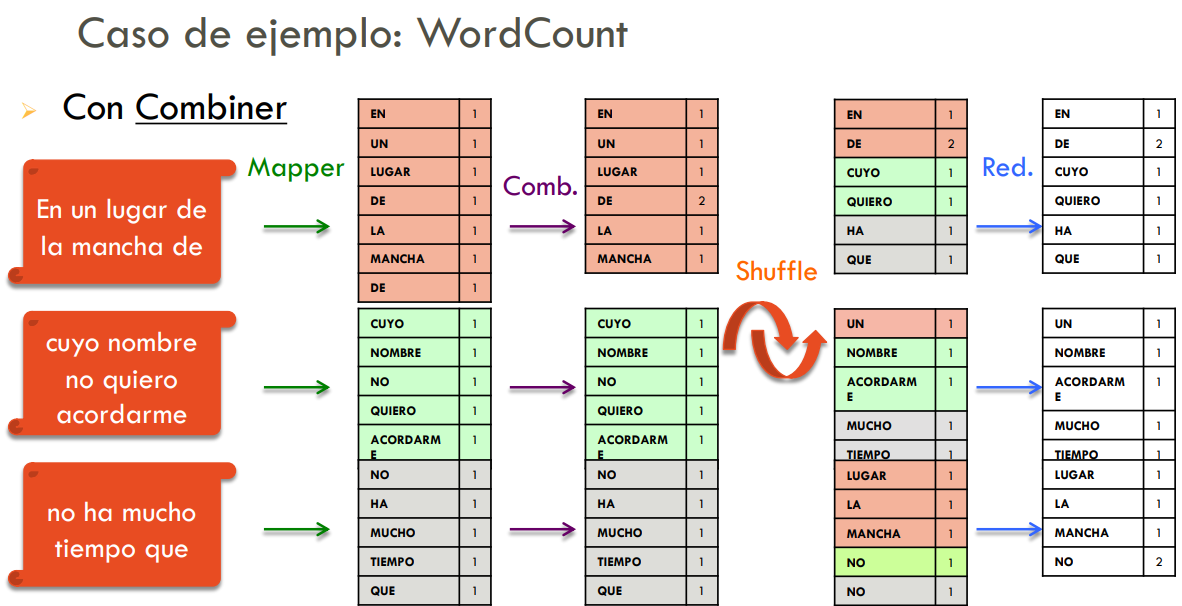
\includegraphics[width=1\linewidth]{figures/MapReduce_example}
\caption{Aplicación Hadoop para el recuento de palabras de el Quijote}
\label{fig:mapreduceexample}
\end{sidewaysfigure}
\break
\subsection{Planificación de un cluster Hadoop}
\textbf{CONSIDERACIONES INICIALES Y ESCALABILIDAD}\\\\
Es recomendable empezar con un clúster pequeño, con los mínimos recursos que sean capaces de cumplir los requerimientos y ampliarlo a medida que escale el problema.\\\\
Por lo general, se debe escalar el clúster cuando:
\begin{itemize}
	\item \textbf{Se necesita mayor capacidad de cómputo}
	\item \textbf{Aumenta el volumen de datos a almacenar.} Cabe señalar que no se debe implementar ninguna estructura RAID en los discos, Hadoop ya viene con un factor de replicación que implementa la redundancia.
	\item \textbf{Aumenta la cantidad de memoria requeria por los procesos a ejecutar}
\end{itemize}
Existen varias reglas de escalado sencillas que pueden orientar la estrategia de crecimiento del clúster:
\begin{itemize}
	\item \textbf{Criterio de Almacenamiento}. HDFS tiene un factor de replicación por defecto igual a 3 que puede modificarse, así es que lo denotaremos como $RF$. Además, se debe añadir un 25\% más de almacenamiento HDFS y hasta un 30\% no HDFS opcional para los ficheros de la propia instancia. Entonces, llamando $VD$ al volumen de datos por unidad de tiempo ($TB/u.t.$), la necesidad de almacenamiento se calcula:
	$$X = 1.55\times RF \times \textrm{VD}$$
	Entonces, si cada servidor tiene una capacidad de almacenamiento $Y \textrm{ TB}$, se debe incorporar una nueva máquina en cada instante dado por el siguiente resultado:
	$$\frac{Y}{X} = \frac{Y}{1.55\times RF \times \textrm{VD}}\textrm{ u.t.}$$
	Por otro lado, es preferible tener un número alto de unidades de almacenamiento para que, en la medida de lo posible, cada tarea acceda a discos distintos y no se sature el proceso de lectura en un conjunto pequeño de discos (usar 8 x 1,5 TB es probablemente mejor que 6 x 2 TB). Además, un máximo adecuado pueden ser 36 TB por nodo, ya que más cantidad impacta en el tráfico de red si un nodo se cae y comienza un proceso de replicación.
	\item \textbf{Criterio de Memoria.} En este caso depende de los demonios que se ejecuten en cada nodo. Se distinguen dos casos:
	\begin{enumerate}
		\item NameNode (Secondary NameNode). Un criterio básico es 2 GB para tareas de gestión del cluster, 2 GB para el procesamiento de metadatos del demonio y 4 GB para procesos del SO.
		\item DataNode. En este caso, depende del número de CPUs del nodo esclavo. Un criterio básico consiste en 
		$\textrm{nº CPUs} \times 4-8 \textrm{ GB}$, 4-8 GB para procesos del demonio, 4-8 GB para el TaskTracker y otros 4 GB para el OS.  
	\end{enumerate}
	Además, conviene evitar el uso de memoria virtual (swap) e implementar umbrales de uso de memoria, ya que se estaría cambiando el alto I/O de la RAM por la lentitud de acceso a disco\footnote{discusión al respecto: \url{https://intelligentsysadmin.wordpress.com/2020/06/23/swap-and-hadoop/}}. 
	\item \textbf{Criterio de Cómputo.} En este caso se recomienda seguir el estándar de CPUs del mercado. A fecha de hoy, basándonos en Intel, se recomienda incorporar CPUs con 6 cores HyperThreading (12 cores lógicos por procesador). Cabe mencionar que los clúster habitualmente vienen limitados por los discos (velocidad I/O) y la latencia de red (velocidad de comunicación entre nodos, clúster-cliente, etc) por lo que no conviene invertir excesivos recursos en CPUs. También, a mayor número de cores, mayor necesidad de almacenamiento y memoria.
\end{itemize}
\textbf{CONSIDERACIONES SOBRE DE VIRTUALIZACIÓN}\\\\
La virtualización supone una penalización de rendimiento y confiabilidad por varios motivos:
\begin{itemize}
	\item Contención de red
	\item Se suelen emplear discos remotos y configurados como un único volumen, aunque
	el disco sea local
	\item No hay modo de garantizar el alojamiento de los nodos en distintos racks, por lo que si falla, se pueden perder conjuntos grandes de nodos.
	\item La redundancia pierde sentido, ya que es posible que los datos se encuentren en la misma máquina física.
\end{itemize}
\textbf{CONSIDERACIONES SOBRE DEL FALLO DE NODOS}\\\\
Se asume que cualquier nodo puede fallar en algún momento, incluído los nodos maestros.\\\\
En caso de fallo de un nodo esclavo, el NameNode replica todos sus datos en otro nodo para mantener el factor de replicación. Por otro lado, el ResouceManager reasignará sus tareas a otros nodos.\\\\
En casa de caer un nodo maestro las consecuencias, si no está en modo Alta Disponibilidad, dependen del demonio que esté ejecutando:
\begin{itemize}
	\item \textbf{NameNode.} Los datos del clúster son inaccesibles, ya que es el demonio que controla qué información tiene cada nodo.
	\item \textbf{ResourceManager.} No se pueden ejecutar tareas, ya que este demonio se encarga de asignarlas entre los nodos.
\end{itemize}
\textbf{CONSIDERACIONES SOBRE DE LA RED}\\\\
Hadoop hace uso intensivo de red, ya que todos los nodos se comunican entre sí. Así, los nodos deberían estar comunicados entre sí con un mínimo de 1 Gbps y se debe considerar 10 Gbps para clústeres con una gran cantidad de datos o que generen gran cantidad de datos intermedios.\\\\
Además, es recomendable usar switches dedicados para el clúster. Los nodos de un mismo rack deben conectarse a switches top-of-rack y los racks a través de core switches de 10 Gbps o más rápidos. \\\\
Para resolver los nombres en la red es recomendable usar nombres propios en lugar de IPs para identificar nodos. Por ejemplo, se puede usar el protocolo DNS. Además, hay que tener en cuenta que Hadoop usa la resolución de nombres directa e inversa. Por ejemplo, si los esclavos se encuentran en una red interna no será posible resolver los nombres desde un cliente externo.\\\\
Se recomienda además deshabilitar el firewall dentro del clúster o permitir acceso total entre máquinas del clúster de cara a evitar problemas de acceso a los nodos. Hadoop emplea muchos puertos de red y es difícil llevar un control.
